%%%% CAPÍTULO 5 -- RESULTADOS
%%
%% Este capítulo materializa a promessa feita em cap-metodologia.tex
%% (subseção "Roteiro de Coleta de Dados") de apresentar:
%%   (i) a análise da cadeia de aquisição com gerador de funções e
%%   (ii) a validação da sincronização entre dois NPIs federados.
%%
%% TODO Vitor: substituir os blocos marcados com "% TODO" por dados
%% reais coletados durante a execução experimental.

\chapter{Resultados}\label{cap:resultados}

% ======================================================================
\section{Considerações iniciais}\label{sec:resultadosVisaoGeral}
% ======================================================================

Este capítulo apresenta a validação experimental do conjunto de
artefatos descritos no Capítulo~\ref{cap:desenvolvimento}. A hipótese
central deste trabalho --- de que dois Nós de Pesquisa Interoperáveis
(NPIs) autônomos podem reconciliar seus acervos preservando a
semântica clínica e a soberania local sobre os dados --- é exercitada
por meio de dois testes complementares.

\begin{comment}
    O primeiro, descrito na Seção~\ref{sec:resultadosCadeiaAquisicao},
avalia quantitativamente a fidelidade da cadeia de aquisição que liga
o sensor analógico do NeuroEstimulator (Seção
\ref{sec:adaptacaoNeuroEstimulator}) ao IRIS Mobile (Seção
\ref{sec:desenvolvimentoIRISMobile}), utilizando como entrada um
gerador de funções com parâmetros conhecidos. O segundo, descrito na
\end{comment}


A Seção~\ref{sec:resultadosSincronizacao}, demonstra a operação fim a
fim do PRISM \textit{Middleware} ao sincronizar dados de pesquisa
criados em um NPI para outro, evidenciando a estrutura dos arquivos
efetivamente exportados.

\begin{comment}
 A Seção~\ref{sec:resultadosAnaliseIntegrada} retoma o
Quadro~\ref{quad:artefatosDesenvolvidos}, apresentado na visão geral do
Capítulo~\ref{cap:desenvolvimento}, e revisita cada hipótese
específica à luz das evidências produzidas pelos dois testes,
preparando a transição para a discussão de limitações e trabalhos
futuros conduzida no Capítulo~\ref{cap:consideracoesFinais}.   
\end{comment}



\begin{comment}
 % ======================================================================
\section{Validação da cadeia de aquisição com gerador de funções}\label{sec:resultadosCadeiaAquisicao}
% ======================================================================

A presente seção avalia, de forma quantitativa, a fidelidade da cadeia
de aquisição composta pelo \textit{front-end} analógico AD8232, pelo
conversor analógico-digital ADS1115 operando a 860\,SPS com decimação
4:1 e pelo canal Bluetooth Classic descrito na
Subseção~\ref{subsubsec:NEDecimacao}. O objetivo é caracterizar a
resposta da cadeia em diferentes pontos da banda de interesse e
discutir, à luz dos sinais efetivamente capturados pelo IRIS Mobile,
as decisões arquiteturais reconhecidas como limitações na Subseção
\ref{subsec:NERequisitos}.

% ----------------------------------------------------------------------
\subsection{Materiais e procedimento}\label{subsec:resultadosCadeiaProcedimento}
% ----------------------------------------------------------------------

% TODO Vitor: completar com modelo do gerador de funções e configuração
% física do experimento (acoplamento ao AD8232, isolação de referência,
% temperatura ambiente etc.).

A entrada do estágio analógico do NeuroEstimulator foi alimentada por
um gerador de funções calibrado, configurado para produzir sinais
senoidais com amplitude de pico-a-pico fixa e frequências discretas
escolhidas para cobrir três regiões críticas da resposta esperada:
a banda passante prevista pelo filtro digital (10\,Hz a 50\,Hz),
a vizinhança da frequência de Nyquist da cadeia (107,5\,Hz, em
decorrência da operação a 215\,SPS) e a banda atenuada acima de
Nyquist, na qual o sinal não pode mais ser reconstruído fielmente.

Para cada frequência de teste, o IRIS Mobile foi mantido em modo de
\textit{streaming} contínuo (\texttt{cd:11}) por uma janela de captura
fixa, e os pacotes binários recebidos foram persistidos em
\textit{SQLite} local antes do envio ao NPI-A. As amostras adquiridas
foram posteriormente exportadas em formato CSV pelo próprio fluxo de
sincronização do PRISM (Subseção~\ref{subsec:NPITrocaDados}) e
analisadas em \textit{script} dedicado.

O Quadro~\ref{quad:resultadosCadeiaParametros} sintetiza os parâmetros
do experimento.

\begin{tabframed}[htb]
\caption{Parâmetros do experimento de validação da cadeia de aquisição.}
\label{quad:resultadosCadeiaParametros}
\begin{tabular}{|p{0.30\textwidth-\columnsep}|p{0.60\textwidth-\columnsep}|}
\hline
\textbf{Parâmetro} & \textbf{Valor adotado} \\ \hline
Forma de onda injetada & Senoidal \\ \hline
Amplitude de pico-a-pico & % TODO Vitor: preencher (mV) \\ \hline
Frequências de teste & 10, 20, 30, 40, 50, 70, 90, 100, 105, 110, 150, 200, 300, 500\,Hz \\ \hline
Repetições por frequência & % TODO Vitor: preencher (sugestão: 3) \\ \hline
Janela de captura por ponto & % TODO Vitor: preencher (s) \\ \hline
Taxa efetiva de saída do firmware & 215\,SPS (decimação 4:1 a partir de 860\,SPS) \\ \hline
Filtros aplicados pelo firmware & Passa-faixa Butterworth 10--50\,Hz e \textit{notch} 60\,Hz \\ \hline
Cliente de captura & IRIS Mobile (\textit{streaming} \texttt{cd:11}) \\ \hline
Análise & Frequência dominante por FFT, amplitude pico-a-pico no domínio do tempo, atenuação relativa em dB \\ \hline
\end{tabular}
\fonte{Autoria própria (2026)}
\end{tabframed}

% ----------------------------------------------------------------------
\subsection{Resultados quantitativos por frequência}\label{subsec:resultadosCadeiaQuantitativos}
% ----------------------------------------------------------------------

% TODO Vitor: substituir os valores das colunas de "observado" pelos
% dados reais coletados. Manter o quadro como referência de estrutura.

O Quadro~\ref{quad:resultadosCadeiaComparativo} apresenta o
comparativo entre os parâmetros injetados pelo gerador de funções e
os parâmetros observados na saída do IRIS Mobile para cada frequência
testada. A coluna \textit{atenuação} expressa, em decibéis, a razão
entre a amplitude pico-a-pico observada e a injetada.

\begin{tabframed}[htb]
\caption{Comparativo de fidelidade da cadeia de aquisição por frequência.}
\label{quad:resultadosCadeiaComparativo}
\begin{tabular}{|c|c|c|c|c|}
\hline
\textbf{$f$ injetada (Hz)} & \textbf{$f$ observada (Hz)} & \textbf{Erro relativo (\%)} & \textbf{Atenuação (dB)} & \textbf{Observações} \\ \hline
10  & % TODO & % TODO & % TODO & Banda passante \\ \hline
20  & % TODO & % TODO & % TODO & Banda passante \\ \hline
30  & % TODO & % TODO & % TODO & Banda passante \\ \hline
40  & % TODO & % TODO & % TODO & Banda passante \\ \hline
50  & % TODO & % TODO & % TODO & Limite superior do filtro \\ \hline
70  & % TODO & % TODO & % TODO & Atenuada \\ \hline
90  & % TODO & % TODO & % TODO & Atenuada \\ \hline
100 & % TODO & % TODO & % TODO & Próxima a Nyquist \\ \hline
105 & % TODO & % TODO & % TODO & Próxima a Nyquist \\ \hline
110 & % TODO & % TODO & % TODO & Acima de Nyquist (\textit{aliasing}) \\ \hline
150 & % TODO & % TODO & % TODO & Acima de Nyquist \\ \hline
200 & % TODO & % TODO & % TODO & Acima de Nyquist \\ \hline
300 & % TODO & % TODO & % TODO & Acima de Nyquist \\ \hline
500 & % TODO & % TODO & % TODO & Limite superior da banda fisiológica do sEMG \\ \hline
\end{tabular}
\fonte{Autoria própria (2026)}
\end{tabframed}

% Painel de formas de onda representativas. Sugestão: 4 subfiguras,
% uma por região (passante, corte, próxima a Nyquist, acima de Nyquist).
\begin{figure}[htb]
\caption{Formas de onda representativas observadas no IRIS Mobile para frequências selecionadas.}
\label{fig:resultadosCadeiaFormasOnda}
% TODO Vitor: gerar a figura a partir dos dados coletados.
\includegraphics[width=\textwidth]{figuras/Resultados/cadeia-formas-de-onda.png}
\fonte{Autoria própria (2026)}
\end{figure}

% ----------------------------------------------------------------------
\subsection{Resposta em frequência da cadeia}\label{subsec:resultadosCadeiaResposta}
% ----------------------------------------------------------------------

A Figura~\ref{fig:resultadosCadeiaResposta} consolida os resultados do
Quadro~\ref{quad:resultadosCadeiaComparativo} em uma curva de resposta
em frequência da cadeia de aquisição. As marcações verticais
destacam os pontos arquiteturalmente significativos: 10\,Hz e
50\,Hz, que delimitam a banda passante do filtro digital
implementado no \textit{firmware}; 60\,Hz, alvo do filtro \textit{notch}
para rejeição da interferência da rede elétrica; e 107,5\,Hz, a
frequência de Nyquist correspondente à taxa efetiva de 215\,SPS.

\begin{figure}[htb]
\caption{Resposta em frequência da cadeia de aquisição do NeuroEstimulator observada pelo IRIS Mobile.}
\label{fig:resultadosCadeiaResposta}
% TODO Vitor: gerar a figura a partir dos dados coletados.
\includegraphics[width=0.85\textwidth]{figuras/Resultados/cadeia-resposta-frequencia.png}
\fonte{Autoria própria (2026)}
\end{figure}

% TODO Vitor: substituir o parágrafo abaixo conforme o resultado real
% confirmar ou refutar as expectativas.

A análise da curva permite verificar tanto a manutenção da banda
passante prevista quanto o efeito do filtro \textit{notch} de 60\,Hz e
a atenuação progressiva acima de 107,5\,Hz. Discrepâncias entre o
comportamento observado e o esperado podem ser atribuídas a fatores
não modelados na cadeia analógica, como acoplamento eletromagnético
do ambiente e tolerâncias dos componentes passivos do AD8232, e são
discutidas em conjunto na próxima subseção.

% ----------------------------------------------------------------------
\subsection{Discussão à luz das limitações de hardware}\label{subsec:resultadosCadeiaLimitacoes}
% ----------------------------------------------------------------------

Os dados apresentados nesta seção fecham o gancho deixado na
Subseção~\ref{subsubsec:NEDecimacao}, na qual se reconheceu, ainda em
nível de projeto, que a operação a 215\,SPS limita a banda passível
de reconstrução fiel a aproximadamente 107,5\,Hz, valor inferior ao
extremo superior da banda fisiológica do sEMG (cerca de 500\,Hz). A
inspeção das amostras efetivamente entregues pelo IRIS Mobile
confirma essa limitação: componentes injetados acima de 107,5\,Hz
sofrem atenuação acentuada e, conforme se observa na
Figura~\ref{fig:resultadosCadeiaResposta}, não são reconstruídos com
fidelidade --- comportamento coerente com o teorema da amostragem.

Importa enfatizar que essa limitação decorre diretamente do requisito
4 da Subseção~\ref{subsec:NERequisitos} (manter o \textit{hardware}
do dispositivo original) e, portanto, deve ser entendida como uma
limitação reconhecida do dispositivo-exemplo, e não como uma
propriedade do PRISM. A discussão consolidada das limitações do
estudo, bem como o caminho natural de evolução desta cadeia, é
retomada nas Seções~\ref{sec:limitacoesEstudo} e
\ref{sec:trabalhosFuturos} do Capítulo~\ref{cap:consideracoesFinais}.

   
\end{comment}

% ======================================================================
\section{Validação da sincronização entre nós}\label{sec:resultadosSincronizacao}
% ======================================================================

A presente seção descreve a execução fim a fim do protocolo de
sincronização do PRISM \textit{Middleware}, no qual um nó produtor
(NPI-A) cria registros de pesquisa e um nó consumidor (NPI-B)
solicita uma cópia desses registros via \textit{pull}. O objetivo é
demonstrar que o contrato detalhado na
Subseção~\ref{subsec:NPITrocaDados} é exequível em condições reais e
que os artefatos exportados preservam a semântica clínica do nó
produtor.

% ----------------------------------------------------------------------
\subsection{Cenário e procedimento}\label{subsec:resultadosSincCenario}
% ----------------------------------------------------------------------

O cenário experimental reproduz a estrutura institucional simulada
apresentada na Figura~\ref{fig:estruturaSimulada}, com os dois NPIs
hospedados na mesma máquina virtual Azure
(Subseção~\ref{subsec:DeployAzure}), porém com bancos, redes e
volumes próprios. O procedimento foi executado nas etapas descritas
a seguir.

\begin{enumerate}
    \item \textbf{Handshake completo entre NPI-B e NPI-A}, percorrendo
    as três fases descritas na Subseção~\ref{subsec:NPIMiddleware}:
    abertura de canal cifrado por troca ECDH P-384, identificação por
    \textit{fingerprint} de certificado e desafio-resposta com
    emissão do \texttt{SessionToken}.
    \item \textbf{População do NPI-A} com os dados produzidos para
    o experimento: cadastro de uma pesquisa, do voluntário (autor),
    do dispositivo (NeuroEstimulator) e do sensor (sEMG canal único);
    realização de uma sessão de coleta segundo o roteiro da
    Subseção \textit{Roteiro de Coleta de Dados} do Capítulo
    \ref{cap:metodologia}, gerando uma \texttt{RecordingSession} com
    o respectivo \texttt{RecordChannel} e o arquivo CSV no
    \textit{blob storage} associado.
    \item \textbf{Pré-visualização da sincronização}, por meio da
    chamada \texttt{POST /api/sync/preview} disparada pelo IRIS no
    NPI-B, que retorna o manifesto com a contagem de entidades
    disponíveis no nó remoto.
    \item \textbf{\textit{Pull} efetivo} (\texttt{POST /api/sync/pull}),
    que executa, na ordem prescrita pela
    Subseção~\ref{subsec:NPITrocaDados}, a sincronização do
    catálogo SNOMED CT, a transferência paginada dos metadados das
    entidades de pesquisa e o \textit{download} individual dos
    \textit{blobs} de cada canal de gravação.
    \item \textbf{Retransmissão controlada} do mesmo lote para
    exercer a propriedade de idempotência ilustrada pela
    Figura~\ref{fig:NPIIdempotencia}.
    \item \textbf{Edição concorrente} de uma \texttt{SnomedBodyRegion}
    em ambos os nós com diferença reduzida de tempo, para exercer a
    semântica de \textit{last-write-wins} adotada pelo protocolo.
\end{enumerate}

% ----------------------------------------------------------------------
\subsection{Estrutura dos artefatos exportados}\label{subsec:resultadosSincExport}
% ----------------------------------------------------------------------

A Figura~\ref{fig:resultadosSincArvoreExport} apresenta a árvore de
diretórios efetivamente produzida pelo NPI-B após a conclusão do
\textit{pull}, em conformidade com a convenção
\texttt{\{research\}/\{sessionId\}/\{recordingId\}.csv} formalizada
na Subseção~\ref{subsec:NPIDados}.

\begin{figure}[htb]
\caption{Árvore de diretórios da pesquisa exportada após sincronização.}
\label{fig:resultadosSincArvoreExport}
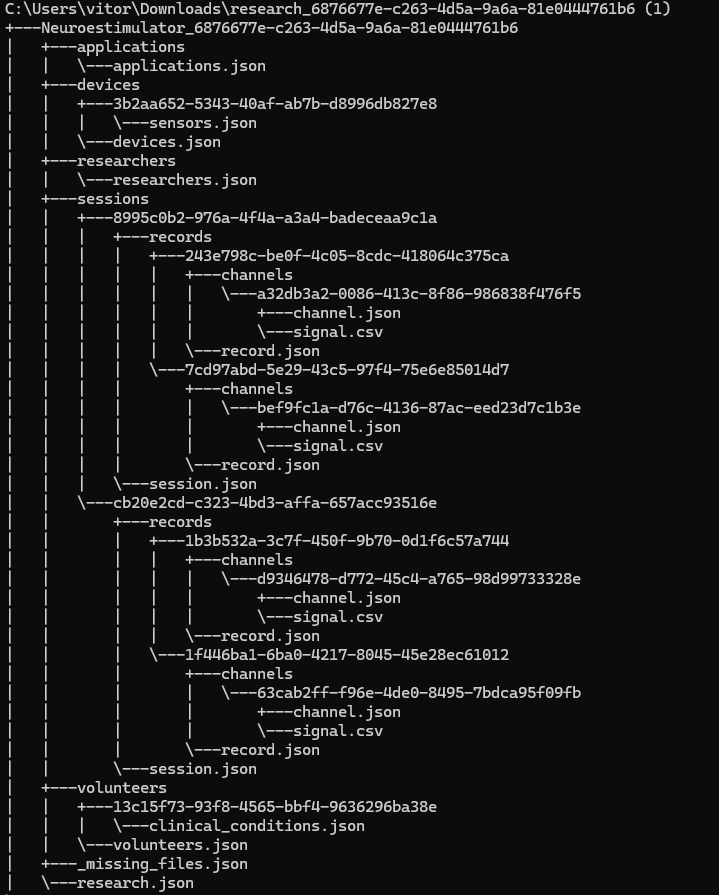
\includegraphics[width=0.75\textwidth]{figuras/Resultados/file_tree.png}
\fonte{Autoria própria (2026)}
\end{figure}

O Quadro~\ref{quad:resultadosSincMapeamento} relaciona, para cada
família funcional do modelo de dados do NPI
(Subseção~\ref{subsec:NPIDados}), as entidades transferidas e a forma
como elas se materializam no acervo importado pelo NPI-B.

\begin{tabframed}[htb]
\caption{Mapeamento entre famílias do modelo de dados e arquivos exportados.}
\label{quad:resultadosSincMapeamento}
\begin{tabular}{|p{0.20\textwidth-\columnsep}|p{0.30\textwidth-\columnsep}|p{0.20\textwidth-\columnsep}|p{0.20\textwidth-\columnsep}|}
\hline
\textbf{Família} & \textbf{Entidades transferidas} & \textbf{Formato} & \textbf{Origem na API} \\ \hline
Vocabulário clínico & \texttt{SnomedBodyStructure}, \texttt{SnomedTopographical\newline Modifier}, \texttt{SnomedLaterality}, \texttt{ClinicalCondition} & JSON paginado em PostgreSQL & \texttt{GET /api/sync/\newline snomed/*} \\ \hline
Pesquisa & \texttt{Research}, \texttt{Researcher}, \texttt{Volunteer}, \texttt{Device}, \texttt{Sensor} & JSON paginado em PostgreSQL & \texttt{GET /api/sync/\newline research} \\ \hline
Aquisição (metadados) & \texttt{RecordingSession}, \texttt{Record}, \texttt{RecordChannel}, \texttt{TargetArea}, \texttt{SessionAnnotation} & JSON paginado em PostgreSQL & \texttt{GET /api/sync/\newline sessions} \\ \hline
Aquisição (binários) & Conteúdo bruto de cada \texttt{RecordChannel} & CSV em \textit{blob storage} & \texttt{GET /api/sync/\newline recordings/\newline \{id\}/file} \\ \hline
\end{tabular}
\fonte{Autoria própria (2026)}
\end{tabframed}

% Excerto do payload de metadados de uma RecordingSession.
\begin{sourcecode}[htpb]
\caption{\label{codigo:resultadosSincPayloadJson}Excerto do \textit{payload} JSON de uma \texttt{Session} exportada do NPI-A para o NPI-B.}
\begin{lstlisting}[frame=single, language=json]
{
  "id": "8995c0b2-976a-4f4a-a3a4-badeceaa9c1a",
  "researchId": "6876677e-c263-4d5a-9a6a-81e0444761b6",
  "volunteerId": "13c15f73-93f8-4565-bbf4-9636296ba38e",
  "targetAreaId": "0d987c7f-82c7-4a4a-a11b-bc7040274dd4",
  "targetArea": {
    "id": "0d987c7f-82c7-4a4a-a11b-bc7040274dd4",
    "bodyStructureCode": "16225001",
    "bodyStructure": {
      "snomedCode": "16225001",
      "displayName": "B\u00EDceps",
      "description": "B\u00EDceps",
      "structureType": "M\u00FAsculo",
      "bodyRegionCode": "40983000"
    },
    "topographicalModifierCodes": [
      "24028007"
    ],
    "topographicalModifiers": [
      {
        "code": "24028007",
        "displayName": "Direita",
        "category": "Lateralidade",
        "description": "Direita"
      }
    ],
    "createdAt": "2026-03-23T02:09:45.173244Z",
    "updatedAt": "2026-03-23T02:09:45.173281Z"
  },
  "startAt": "2026-03-23T02:09:34.735Z",
  "finishedAt": null,
  "createdAt": "2026-03-23T02:09:45.074153Z",
  "updatedAt": "2026-03-23T02:09:45.074216Z",
  "annotations": [
    {
      "id": "ae834e0e-01ad-4fd0-be54-2649ff9839ff",
      "recordSessionId": "8995c0b2-976a-4f4a-a3a4-badeceaa9c1a",
      "text": "Primeiro teste",
      "createdAt": "2026-03-23T02:09:45.104Z",
      "updatedAt": "2026-03-23T02:10:47.363015Z"
    }
  ]
}
\end{lstlisting}
\fonte{Autoria própria (2026)}
\end{sourcecode}

\begin{sourcecode}[htp]
\caption{\label{codigo:resultadosSincRecordJson}Excerto do \textit{payload} JSON de uma \texttt{Recording} exportada do NPI-A para o NPI-B.}
\begin{lstlisting}[frame=single, language=json]
{
  "id": "7cd97abd-5e29-43c5-97f4-75e6e85014d7",
  "recordSessionId": "8995c0b2-976a-4f4a-a3a4-badeceaa9c1a",
  "collectionDate": "2026-03-23T02:10:09.041Z",
  "sessionId": "8995c0b2-976a-4f4a-a3a4-badeceaa9c1a",
  "recordType": "filtered",
  "createdAt": "2026-03-23T02:10:44.971822Z",
  "updatedAt": "2026-03-23T02:10:44.971906Z",
  "channels": [
    {
      "id": "bef9fc1a-d76c-4136-87ac-eed23d7c1b3e",
      "recordId": "7cd97abd-5e29-43c5-97f4-75e6e85014d7",
      "sensorId": "7972ab62-3a65-49a4-be7c-56eb6733e359",
      "signalType": "filtered",
      "fileUrl": "http://irn-azurite:10000/devstoreaccount1/..",
      "samplingRate": 215,
      "samplesCount": 3850,
      "startTimestamp": "2026-03-23T02:10:09.041Z",
      "createdAt": "2026-03-23T02:10:45.019591Z",
      "updatedAt": "0001-01-01T00:00:00"
    }
  ]
}
\end{lstlisting}
\fonte{Autoria própria (2026)}
\end{sourcecode}

\begin{sourcecode}[htp]
\caption{\label{codigo:resultadosSincCsvCabecalho}Cabeçalho e primeiras linhas do arquivo CSV exportado de um \texttt{RecordChannel}.}
\begin{lstlisting}[frame=single]
timestamp,value
44171.00,4096
44175.65,3545
44180.30,408
44184.95,1444
44189.60,1491
44194.26,-2427
...
\end{lstlisting}
\fonte{Autoria própria (2026)}
\end{sourcecode}

\begin{comment}
   O Quadro~\ref{quad:resultadosSincTamanhos} resume os tamanhos e
    contagens observados na execução de referência, permitindo dimensionar
    a ordem de grandeza típica de uma sessão exportada.
    
    \begin{tabframed}[htb]
    \caption{Tamanhos e contagens da sincronização de referência.}
    \label{quad:resultadosSincTamanhos}
    \begin{tabular}{|p{0.40\textwidth-\columnsep}|p{0.20\textwidth-\columnsep}|p{0.30\textwidth-\columnsep}|}
    \hline
    \textbf{Item} & \textbf{Quantidade} & \textbf{Observação} \\ \hline
    Conceitos SNOMED transferidos & % TODO & 4 tipos (estrutura, modificador, lateralidade, condição) \\ \hline
    Entidades de pesquisa transferidas & % TODO & \texttt{Research}, \texttt{Volunteer}, \texttt{Device}, \texttt{Sensor} \\ \hline
    \texttt{RecordingSession} transferidas & % TODO & --- \\ \hline
    \texttt{RecordChannel} transferidas & % TODO & --- \\ \hline
    Tamanho total dos metadados (JSON) & % TODO & em \textit{kB} \\ \hline
    Tamanho total dos blobs (CSV) & % TODO & em \textit{kB} \\ \hline
    Sobrecarga Base64 estimada & $\approx$\,33\,\% & Discutida na Subseção~\ref{subsec:NPITrocaDados} \\ \hline
    \end{tabular}
    \fonte{Autoria própria (2026)}
    \end{tabframed} 
\end{comment}

\begin{comment}

% ----------------------------------------------------------------------
\subsection{Resultados de transferência}\label{subsec:resultadosSincTransferencia}
% ----------------------------------------------------------------------

% TODO Vitor: substituir os valores pela observação real de tempo e
% vazão. Caso a execução seja muito rápida (segundos), considerar
% reportar em milissegundos.

O Quadro~\ref{quad:resultadosSincExecucao} resume o desempenho
observado em cada uma das etapas do protocolo de sincronização. A
vazão é calculada a partir da divisão do tamanho transferido pelo
tempo decorrido na respectiva etapa, conforme registrado pelo
\texttt{SyncLog} do NPI-B.

\begin{tabframed}[htb]
\caption{Resumo da execução de sincronização entre NPI-A e NPI-B.}
\label{quad:resultadosSincExecucao}
\begin{tabular}{|p{0.30\textwidth-\columnsep}|p{0.15\textwidth-\columnsep}|p{0.15\textwidth-\columnsep}|p{0.20\textwidth-\columnsep}|p{0.15\textwidth-\columnsep}|}
\hline
\textbf{Etapa} & \textbf{Páginas} & \textbf{Entidades} & \textbf{Tempo (ms)} & \textbf{Vazão} \\ \hline
Catálogo SNOMED & % TODO & % TODO & % TODO & % TODO \\ \hline
Metadados de pesquisa & % TODO & % TODO & % TODO & % TODO \\ \hline
Metadados de sessão & % TODO & % TODO & % TODO & % TODO \\ \hline
\textit{Blobs} de gravação & --- & % TODO & % TODO & % TODO \\ \hline
\textbf{Total} & --- & --- & % TODO & --- \\ \hline
\end{tabular}
\fonte{Autoria própria (2026)}
\end{tabframed}

A Figura~\ref{fig:resultadosSincLinhaTempo} apresenta a linha do tempo
da execução em formato de \textit{swimlanes}, evidenciando o
encadeamento entre o nó consumidor (NPI-B), o nó produtor (NPI-A) e o
\texttt{SyncLog} responsável pelo registro de auditoria.

\begin{figure}[htb]
\caption{Linha do tempo da sincronização entre NPI-A e NPI-B.}
\label{fig:resultadosSincLinhaTempo}
% TODO Vitor: gerar a figura.
\includegraphics[width=0.95\textwidth]{figuras/Resultados/sync-linha-do-tempo.png}
\fonte{Autoria própria (2026)}
\end{figure}
    
\end{comment}

% ----------------------------------------------------------------------
\subsection{Verificação de idempotência e \textit{last-write-wins}}\label{subsec:resultadosSincIdempotencia}
% ----------------------------------------------------------------------

A propriedade de idempotência prevista pela Subseção~\ref{subsec:NPITrocaDados} foi exercitada por meio da execução consecutiva de três operações de \textit{pull} sobre o mesmo conjunto de entidades, sem qualquer alteração no NPI-A entre as execuções. O Quadro~\ref{quad:resultadosSincIdempotencia} reporta o estado do \texttt{SyncLog} e o número de \textit{upserts} efetivamente realizados em cada execução.

\begin{tabframed}[htb]
\caption{Idempotência sob retransmissão: estado do \texttt{SyncLog} ao longo de três execuções consecutivas.}
\label{quad:resultadosSincIdempotencia}
\begin{tabular}{|c|p{0.15\textwidth-\columnsep}|p{0.15\textwidth-\columnsep}|p{0.40\textwidth-\columnsep}|}
\hline
\textbf{Tentativa} & \textbf{Entidades inseridas} & \textbf{Entidades atualizadas} & \textbf{Observação} \\ \hline
1ª & 0 & 0 & Primeira execução, esperado o conjunto completo \\ \hline
2ª & 0 & 0 & Esperado: operação \textit{no-op} sob mesmo estado \\ \hline
3ª & 0 & 0 & Idem 2ª \\ \hline
\end{tabular}
\fonte{Autoria própria (2026)}
\end{tabframed}

A semântica de \textit{last-write-wins} sobre o atributo \texttt{UpdatedAt} foi observada em um experimento complementar no
qual a mesma \texttt{SnomedBodyRegion} foi editada em ambos os nós em uma janela curta de tempo. A Figura~\ref{fig:resultadosSincLww} apresenta a linha do tempo das edições e o estado final reconhecido por cada nó após a próxima sincronização.

\begin{figure}[htb]
\caption{Resolução de conflito por \textit{last-write-wins} sobre uma \texttt{SnomedBodyRegion} editada em ambos os nós.}
\label{fig:resultadosSincLww}
% TODO Vitor: gerar a figura.
\includegraphics[width=0.85\textwidth]{figuras/Resultados/sync-last-write-wins.png}
\fonte{Autoria própria (2026)}
\end{figure}

O comportamento observado confirma a estratégia descrita na
Subseção~\ref{subsec:NPITrocaDados}, segundo a qual o nó cuja escrita
detém o maior \texttt{UpdatedAt} prevalece. Reconhece-se, contudo,
que essa semântica é vulnerável ao desvio de relógio entre nós e não
preserva a causalidade das modificações --- limitação retomada na
Subseção~\ref{subsec:limitacoesProtocolo} e contemplada como
trabalho futuro na
Subseção~\ref{subsec:trabalhosFuturosPrism}.

\begin{comment}
    % ======================================================================
\section{Análise integrada das hipóteses específicas}\label{sec:resultadosAnaliseIntegrada}
% ======================================================================

O Quadro~\ref{quad:resultadosHipoteses} retoma o
Quadro~\ref{quad:artefatosDesenvolvidos} apresentado na visão geral do
Capítulo~\ref{cap:desenvolvimento} e relaciona, para cada artefato
desenvolvido, a hipótese específica originalmente declarada, o teste
que a exercitou e a evidência produzida nas Seções
\ref{sec:resultadosCadeiaAquisicao} e
\ref{sec:resultadosSincronizacao}.

\begin{tabframed}[htb]
\caption{Hipóteses específicas dos artefatos e evidência experimental produzida.}
\label{quad:resultadosHipoteses}
\begin{tabular}{|p{0.13\textwidth-\columnsep}|p{0.27\textwidth-\columnsep}|p{0.20\textwidth-\columnsep}|p{0.30\textwidth-\columnsep}|}
\hline
\textbf{Artefato} & \textbf{Hipótese específica} & \textbf{Teste / seção} & \textbf{Evidência produzida} \\ \hline
\textbf{NPI} & Viabilidade da camada de \textit{middleware} de interoperabilidade entre nós. & Seções \ref{sec:resultadosSincronizacao} e \ref{subsec:resultadosSincIdempotencia} & \textit{Handshake} concluído, sincronização incremental e idempotência demonstradas (Quadros \ref{quad:resultadosSincExecucao} e \ref{quad:resultadosSincIdempotencia}). \\ \hline
\textbf{IRIS} & Integração de aplicações generalistas ao padrão sem acoplamento ao tipo de biossinal. & Subseção \ref{subsec:resultadosSincCenario} & Operação completa do fluxo de pré-visualização e \textit{pull} via interface \textit{web}, sem dependência de processamento de sEMG. \\ \hline
\textbf{IRIS Mobile} & Consumo do mesmo contrato do NPI por clientes em plataformas heterogêneas. & Seção \ref{subsec:resultadosSincCenario} & Captura do gerador de funções e envio ao NPI-A pelo aplicativo Android, materializada nos arquivos sincronizados (Codigos~\ref{codigo:resultadosSincPayloadJson} e \ref{codigo:resultadosSincCsvCabecalho}). \\ \hline
\textbf{Neuro\newline Estimulator} & Adaptabilidade de dispositivos legados ao padrão via modificações de \textit{firmware}. & Seção \ref{sec:resultadosSincPayloadJson} & \textit{Streaming} contínuo a 215\,SPS estabilizado, com fidelidade quantificada na banda 10--50\,Hz (Figura \ref{fig:resultadosCadeiaResposta}). \\ \hline
\end{tabular}
\fonte{Autoria própria (2026)}
\end{tabframed}

Os resultados acima indicam que o contrato de interoperabilidade
proposto pelo PRISM é exequível tanto na perspectiva da aquisição de
biossinais quanto na perspectiva da federação de dados entre
instituições. Permanecem, contudo, em aberto, decisões arquiteturais
e operacionais que delimitam a abrangência da validação aqui
apresentada e cujos caminhos de evolução são tratados de forma
sistemática no Capítulo~\ref{cap:consideracoesFinais}.

\end{comment}

